% Template article for preprint document class `elsart'
% SP 2001/01/05
% Modified CG (ESME) for Model 3, single column, 2 titles, abstract/r�sum�,
%  and 2 sets of keywords - 07.01.03 - file called Maths-English.tex
% English Version for Mathematics (CRAS series 1)
% Revamped, CG, 17.08.04, adding header, dates, and presenter

\documentclass{elsart3-1}

% Use the option doublespacing or reviewcopy to obtain double line spacing
% \documentclass[doublespacing]{elsart}

% if you use PostScript figures in your article
% use the graphics package for simple commands
% \usepackage{graphics}
% or use the graphicx package for more complicated commands
% \usepackage{graphicx}
% or use the epsfig package if you prefer to use the old commands
% \usepackage{epsfig}

% The amssymb package provides various useful mathematical symbols
\usepackage{amsmath,amssymb}
\usepackage{graphicx}

\usepackage{color} % TO REMOVE AFTER REVIEW APPROVES COMMENTS IN BLUE

\usepackage[english,francais]{babel}

%ENVIRONMENTS THEOREMS...
% These are predefined, and follow the numbering system used in the journal!
%English
\newtheorem{theorem}{Theorem}[section]
\newtheorem{lemma}[theorem]{Lemma}
\newtheorem{e-proposition}[theorem]{Proposition}
\newtheorem{corollary}[theorem]{Corollary}
\newtheorem{e-definition}[theorem]{Definition\rm}
\newtheorem{remark}{\it Remark\/}
\newtheorem{example}{\it Example\/}
%French
\newtheorem{theoreme}{Th\'eor\`eme}[section]
\newtheorem{lemme}[theoreme]{Lemme}
\newtheorem{proposition}[theoreme]{Proposition}
\newtheorem{corollaire}[theoreme]{Corollaire}
\newtheorem{definition}[theoreme]{D\'efinition\rm}
\newtheorem{remarque}{\it Remarque}
\newtheorem{exemple}{\it Exemple\/}
\renewcommand{\theequation}{\arabic{equation}}
\setcounter{equation}{0}

\newcommand{\fudge}{\fC}
\newcommand{\dtf}{\textit{\doubletilde{f}}}
\newcommand{\cube}{[0,1)^s}
\newcommand{\rf}{\mathring{f}}
\newcommand{\rnu}{\mathring{\nu}}
\newcommand{\natm}{\naturals_{0,m}}
\newcommand{\wcS}{\widecheck{S}}
\newcommand{\tol}{\text{tol}}
\newcommand{\bvec}[1]{\boldsymbol{#1}}
\newcommand{\vi}{\bvec{i}}
\newcommand{\vj}{\bvec{j}}
\newcommand{\ve}{\bvec{e}}
\newcommand{\vk}{\bvec{k}}
\newcommand{\vv}{\bvec{v}}
\newcommand{\vx}{\bvec{x}}
\newcommand{\vz}{\bvec{z}}
\newcommand{\dif}{\mathsf{d}}
\newcommand{\hf}{\hat{f}}
\newcommand{\hS}{\widehat{S}}
\newcommand{\tS}{\widetilde{S}}
\newcommand{\tf}{\tilde{f}}
\newcommand{\fC}{\mathfrak{C}}
\newcommand{\homega}{\widehat{\omega}}
\newcommand{\wcomega}{\mathring{\omega}}
\newcommand{\vzero}{\bvec{0}}
\newcommand{\integers}{\mathbb{Z}}
\newcommand{\naturals}{\mathbb{N}}
\newcommand{\ip}[3][{}]{\ensuremath{\left \langle #2, #3 \right \rangle_{#1}}}

\def\abs#1{\ensuremath{\left \lvert #1 \right \rvert}}

%%%%%%%%%%%%%%%%%%%%%%%%%%%%%%%%
%% GUILLEMETS (FRENCH QUOTES) %%
%%%%%%%%%%%%%%%%%%%%%%%%%%%%%%%%
\def\og{\leavevmode\raise.3ex\hbox{$\scriptscriptstyle\langle\!\langle$~}}
\def\fg{\leavevmode\raise.3ex\hbox{~$\!\scriptscriptstyle\,\rangle\!\rangle$}}


\journal{the Acad\'emie des sciences}
\begin{document}
% place in the next line the header (rubrique) chosen for your article,
% if you know it (you can also have 2, format : Header1/Header2
\centerline{}
\begin{frontmatter}

% Title, authors and addresses

% use the thanksref command within \title, \author or \address for footnotes;
% use the ead command for the email address,
% and the form \ead[url] for the home page:
% \title{Title\thanksref{label1}}
% \thanks[label1]{}
% \author{Name\thanksref{label2}}
% \ead{email address}
% \ead[url]{home page}
% \thanks[label2]{}
% \address{Address\thanksref{label3}}
% \thanks[label3]{}
\selectlanguage{english}
\title{Iterative construction of replicated designs based on Sobol' sequences}
%\title{Replicated designs based on Sobol' sequences to estimate main effects of model inputs}
%\title{On the replication of Sobol' sequences to estimate main effects of model inputs}


% use optional labels to link authors explicitly to addresses:
% \author[label1,label2]{}
% \address[label1]{}
% \address[label2]{}
% The [label1] can be suppressed if there is only one address for all authors

\selectlanguage{english}
\author[authorlabel1]{Laurent Gilquin},
\ead{laurent.gilquin@inria.fr}
\author[authorlabel2]{Llu\'{i}s Antoni Jim\'{e}nez Rugama},
\ead{ljimene1@hawk.iit.edu}
\author[authorlabel3]{Elise Arnaud},
\author[authorlabel2]{Fred J. Hickernell},
\author[authorlabel4]{Herv\'{e} Monod},
\author[authorlabel3]{Cl\'{e}mentine Prieur}

\address[authorlabel1]{Inria Grenoble - Rh\^{o}ne-Alpes, Inovall\'{e}e, 655 avenue de l'Europe, 38330 Montbonnot}
\address[authorlabel2]{Illinois Institute of Technology, Rettaliata Engineering Center, 10 W 32st, Chicago, IL 60616}
\address[authorlabel3]{Univ. Grenoble Alpes, Jean Kunzmann Laboratory, F-38000 Grenoble, France \\
CNRS, LJK, F-38000 Grenoble, France, Inria}
\address[authorlabel4]{MaIAGE, INRA, Universit\'{e} Paris-Saclay, 78350 Jouy-En-Josas, France}

% If you know the dates of reception, and acceptation you can put them now;
%  idem the name of the person presenting the Note

\medskip
\begin{center}
{\small Received *****; accepted after revision +++++\\
Presented by �����}
\end{center}

\begin{abstract}
\selectlanguage{english}
% Text of abstract in English
In the perspective of estimating main effects of model inputs, two approaches are studied to iteratively construct replicated designs based on Sobol' sequences. Space-filling properties of the resulting designs are studied based on two criteria.
{\it To cite this article: L.
Gilquin, Ll. A. Jim\'enez Rugama, E. Arnaud, F. J. Hickernell, H. Monod, C. Prieur, C. R. Acad. Sci. Paris, Ser. I 340 (2016).}

\vskip 0.5\baselineskip

\selectlanguage{francais}
% Text of abstract in French
\noindent{\bf R\'esum\'e} \vskip 0.5\baselineskip \noindent
{ \bf Construction de plans r\'epliqu\'es \`a partir de s\'equences de Sobol'.}
%{\bf Plans r\'epliqu\'es \`a base de s\'equences de Sobol' pour estimer les effets principaux des param\`etres d'un mod\`ele. }
Dans l'objectif d'estimer les effets principaux des param\`etres d'un mod\`ele, nous proposons d'\'etudier deux approches pour construire it\'erativement des plans r\'epliqu\'es \`a partir de s\'equences de Sobol'. Les propri\'et\'es de remplissement de l'espace des plans construits sont \'etudi\'ees sur la base de deux crit\`eres.
{\it Pour citer cet article~: L. Gilquin, Ll. A. Jim\'enez Rugama, E. Arnaud, F. J. Hickernell, H. Monod, C. Prieur, C. R. Acad. Sci.
Paris, Ser. I 340 (2016).}
\end{abstract}
\end{frontmatter}
\selectlanguage{english}
\section{Introduction}
Mathematical models often involve a substantial number of poorly known parameters. The effect of these parameters on the output of the model can be assessed through sensitivity analysis. Global sensitivity analysis methods are useful tools to identify the parameters having the most influence on the output. A well known approach is the variance based method introduced by Sobol' in \cite{Sobol2}. This method estimates sensitivity indices called Sobol' indices that summarize the influence of each model input. Among all Sobol' indices, one can distinguish the first-order indices that estimate the main effect of each input.

The procedure to estimate first-order Sobol' indices proposed by Sobol' and its improvements (see Saltelli \cite{Saltelli} for an exhaustive survey) all suffer from a prohibitive number of model evaluations that grows with respect to the input space dimension. %An elegant solution to reduce this cost relies on the construction of replicated designs introduced by McKay \cite{mckay}.  
 An elegant solution to reduce this number relies on the construction of particular designs of experiments called replicated designs. The notion of replicated designs was first introduced by McKay through its definition of replicated Latin Hypercubes in \cite{Mckay}. Below we provide this definition in a more general framework:

\begin{e-definition}%[Replicated designs]
\label{rep.designs}
Consider $\vx \in [0,1)^s$, and $\vx_u \in [0,1)^{|u|}$ the subset of elements of $\vx$ given by $u\subsetneq \{1,\dots,s\}$, where $|u|$ is the cardinality of $u$. Let $\mathcal{P}=\{\vx_i\}_{i=0}^{n-1}$ and $\mathcal{P}'=\{{\vx'}_i\}_{i=0}^{n-1}$ be two point sets in $[0,1)^{s}$, and denote by $\mathcal{P}^u=\{\vx_{i,u}\}_{i=0}^{n-1}$ (resp. $\mathcal{P}'^u$) the subset of elements of points in $\mathcal{P}$ (resp. $\mathcal{P}'$) indexed by $u$. We say that $\mathcal{P}$ and $\mathcal{P}'$ are two replicated designs of order $a=1,\dots,s-1$, if for any $u\subsetneq \{1,\dots,s\}$ with $|u|=a$, $\mathcal{P}^u$ and $\mathcal{P}'^u$ are the same point set in $[0,1)^a$, perhaps in a different order.
\end{e-definition}

The replication procedure described in \cite{Mara,Tissot} allows the estimation of all first-order Sobol' indices with only two replicated designs of order $1$. This procedure has the major advantage of reducing the number of model evaluations, evaluating only on designs $\mathcal{P}$ and $\mathcal{P}'$ regardless of the input space dimension. However, Sobol' indices estimates may still not be accurate enough if designs $\mathcal{P}$ and $\mathcal{P}'$ do not explore the input space properly.
\bigskip

In this note, we propose two different constructions of replicated designs of order $1$ based on Sobol' sequences. Both constructions ensure that the input space is properly explored and can be used within the replication procedure to estimate all first-order Sobol' indices. The definition of these constructions is recursive, therefore one can iteratively refine each replicated design by adding the corresponding new set of points. We first provide a brief introduction on digital sequences and then present two iterative approaches to construct the two replicated point sets. We end this note by analyzing the space-filling properties of the two designs constructed.

\section{Digital sequences background}

\subsection{Preliminaries}
Digital nets and sequences were first introduced by Niederreiter \cite{Niederreiter} in the numerical integration framework to define good uniformly distributed points in $\cube$. They can also appear in the literature as digital $(t,m,s)$-nets and digital $(t,s)$-sequences, or simply $(t,m,s)$-nets and $(t,s)$-sequences. Sobol' and Niederreiter-Xing sequences are two examples of digital sequences detailed in \cite{Sobol1} and \cite{NiederreiterXing}.

%The quality of any $(t,m,s)$-net or $(t,s)$-sequence is measured by $t$, called the $t$-value. The $t$-value is introduced in the $(t,m,s)$-net definition as follows:

\begin{e-definition}%[$(t,m,s)-net$]
Let $\mathcal{A}$ be the set of all elementary intervals $A\subset \cube$ where $A=\prod_{j=1}^s [\alpha_jb^{-\gamma_j},(\alpha_j+1)b^{-\gamma_j})$, with integers $s\geq 1$, $b\geq 2$, $\gamma_j\geq 0$, and $b^{\gamma_j}>\alpha_j\geq 0$. For $m\geq t\geq 0$, the point set $\mathcal{P}\in\cube$ with $b^m$ points is a $(t,m,s)-net$ in base $b$ if every $A$ with volume $b^{t-m}$ contains $b^t$ points of $\mathcal{P}$.
\end{e-definition}

Thus, a $(t,m,s)$-net is defined such that all elementary intervals of volume $b^{t-m}$ will enclose the same proportion of points of $\mathcal{P}$, namely $b^{t-m}|\mathcal{P}|$ points. The most evenly spread nets are $(0,m,s)$-nets, since each elementary interval of the smallest volume possible, $b^{-m}$, contains exactly one point. The quality of any $(t,m,s)$-net is therefore measured by the parameter $t$, called $t$-value.

By increasing $m$, we increase the number of points of the $(t,m,s)$-net. In the limiting case where $m\rightarrow\infty$, we can define the $(t,s)$-sequence as:
\begin{e-definition}%[$(t,s)$-sequence]
For integers $s\geq 1$, $b\geq 2$, and $t\geq 0$, the sequence $\{\vx_i\}_{i\in\mathbb{N}_0}$ is a $(t,s)$-sequence in base $b$, if for every set $\mathcal{P}_{\ell,m}=\{\vx_i\}_{i=\ell b^m}^{(\ell+1)b^m-1}$ with $\ell\geq 0$ and $m\geq t$, $\mathcal{P}_{\ell,m}$ is a $(t,m,s)$-net in base $b$.
\end{e-definition}

The replicated design properties can also apply to digital sequences. Hence, we introduce the following definition,
\begin{e-definition}
Two digital sequences $\{\vx_i\}_{i\in\mathbb{N}_0}$ and $\{{\vx'}_i\}_{i\in\mathbb{N}_0}$ are \emph{digitally replicated} of order $a$ if for all $m\geq 0$, $\{{\vx}_i\}_{i=0}^{b^m-1}$ and $\{{\vx'}_i\}_{i=0}^{b^m-1}$ are two replicated designs of order $a$.
\end{e-definition}

\subsection{Sobol' sequences}

Sobol' sequences in dimension $s$ are digital sequences in base $b=2$ that can be computed using the \emph{generating matrices}, a set of $s$ full rank infinite dimensional upper triangular matrices over the Galois field $\mathbb{F}_2:=\{0,1\}$.
%We will denote by $\oplus$ the addition in $\mathbb{F}_2$.
These generating matrices are recursively constructed given some primitive polynomials and initial directional numbers. In \cite{Kuo}, Kuo and Joe detail this construction and also suggest a particular choice for these matrices that optimize the 2 dimensional projection $t$-values.

Consider the generating matrices $C_1,\dots,C_s$, and $C_1^m,\dots,C_s^m$ their upper left corner blocks of size $m\times m$. Although $C_1,\dots,C_s$ are of infinite size, one only requires the knowledge of $C_1^m,\dots,C_s^m$ to construct the first $2^m$ Sobol' points: for each $i=0,\dots,2^m-1$, the point $\vx_i = (x_{i,1},\dots,x_{i,s})^\intercal$ of the sequence is obtained dimension-wise by:
\begin{equation}
\label{dig.net.eq.}
(x_{i,j,1},\dots,x_{i,j,m})^\intercal = C_j^{m} \vi,\qquad j= 1,\dots,s\, ,
\end{equation}
where $x_{i,j} = \sum_{k \geq 1}^m x_{i,j,k}2^{-k}$ is the binary expansion of $x_{i,j}$ and $\vi = (i_{0},\dots,i_{m-1})^\intercal$ is the vector obtained from the binary expansion of $i= \sum_{k \geq 0}^{m-1} i_{k}2^{k}$. All matrix operations are performed in $\mathbb{F}_2$. Below we provide an example of how to compute $x_{11,1}=0.8125$ and $x_{9,2}=0.4375$,
\begin{equation*}
\renewcommand{\arraystretch}{1.3}
\begin{pmatrix}
x_{11,1,1} \\
x_{11,1,2} \\
x_{11,1,3} \\
x_{11,1,4}
\end{pmatrix} = 
\underbrace{
\begin{pmatrix}
1 & 0 & 0 & 0 \\
0 & 1 & 0 & 0 \\
0 & 0 & 1 & 0 \\
0 & 0 & 0 & 1
\end{pmatrix}}_{C_1^4}
\underbrace{
\begin{pmatrix}
1 \\
1 \\
0 \\
1
\end{pmatrix}}_{\bvec{11}}=
\begin{pmatrix}
1 \\
1 \\
0 \\
1
\end{pmatrix}
,\qquad
\begin{pmatrix}
x_{9,2,1} \\
x_{9,2,2} \\
x_{9,2,3} \\
x_{9,2,4}
\end{pmatrix} = 
\underbrace{\begin{pmatrix}
1 & 1 & 1 & 1 \\
0 & 1 & 0 & 1 \\
0 & 0 & 1 & 1 \\
0 & 0 & 0 & 1
\end{pmatrix}}_{C_2^4}
\underbrace{\begin{pmatrix}
1 \\
0 \\
0 \\
1
\end{pmatrix}}_{\bvec{9}} =
\begin{pmatrix}
0 \\
1 \\
1 \\
1
\end{pmatrix}
\end{equation*}

%\bigskip

To compute the next $2^m$ points of the sequence, one can infer from \eqref{dig.net.eq.} that
\begin{equation}\label{Sobol_iter_constr}
(x_{i+2^m,j,1},\dots,x_{i+2^m,j,m+1})^\intercal=(x_{i,j,1},\dots,x_{i,j,m},0)^\intercal\oplus {(c_j^{m+1})}^\intercal,\quad i=0,\dots,2^m-1,
\end{equation}
where $c_j^{m+1}$ is the last column of $C_j^{m+1}$ and $\oplus$ is the addition in $\mathbb{F}_2$.

In addition, Sobol' sequences have good group structure properties. For any $m\geq 1$, the first $2^m$ points of the sequence form an Abelian group under $\oplus$:
\begin{equation}
\begin{gathered}
\vx = \left(\sum_{k=1}^m x_{1,k}2^{-k},\dots,\sum_{k=1}^m x_{s,k}2^{-k}\right)^\intercal\; , \qquad \vz = \left(\sum_{k=1}^m z_{1,k}2^{-k},\dots,\sum_{k=1}^m z_{s,k}2^{-k}\right)^\intercal, \\
\vx\oplus\vz := \left(\sum_{k=1}^m (x_{1,k}+z_{1,k}\mod 2)2^{-k},\dots,\sum_{k=1}^m (x_{s,k}+z_{s,k}\mod 2)2^{-k}\right)^\intercal.
\end{gathered}
\label{group.operation}
\end{equation}
From equation \eqref{dig.net.eq.} above, one may see that the first $2^m$ points of the sequence are elements of $\left(\mathbb{F}_2^m\right)^s$.




\begin{lemma}\label{Sobol_replicated}
All Sobol' sequences are digitally replicated of order 1.
\end{lemma}
\textit{Proof}: Consider any two $s$-dimensional Sobol' sequences generated by $C_1,\dots,C_s$ and $C'_1,\dots,C'_s$ respectively. Since any two matrices $C^{m}_j$ and ${C'}^{m}_j$ are square and full rank, the operations $\vi \mapsto C^{m}_j\vi$ and $\vi \mapsto {C'}^{m}_j\vi$ are one-to one and onto for all $i=0,\dots,2^m-1$. Therefore, they generate the same point sets.

%\begin{remark}
%For any $j \in \{1,\dots,s\}$, using two different generating matrices $C^{m}_j$ and $C'^{m}_j$ in equation (\ref{dig.net.eq.}) produce the same set of $2^m$ values $\{x_{0,j},\dots,x_{2^m-1,j}\}$ but ordered differently. It is possible to go from an order to the other by using the corresponding full rank upper triangular matrix $U^{m}_j$, such that $C^{m}_j=C'^{m}U^{m}_j$. This matrix can be thought as a permutation of the input binary vectors $\vi$.
%\end{remark}

%\section{Iterative constructions of extensible replicated point sets of order 1}
\section{Iterative constructions of replicated point sets}

In this section we propose two different approaches to iteratively construct two replicated point sets, $\mathcal{P}_\ell$ and $\mathcal{P}'_\ell$, based on Sobol' sequences. These two constructions are carried out according to the following recursive scheme :
$$\left\lbrace \begin{array}{l}
\mathcal{P}_0= B_0 \\
\mathcal{P}_\ell= \mathcal{P}_{\ell-1} \cup B_\ell \end{array}\right. \,
\hspace*{0.5cm}
\left\lbrace \begin{array}{l}
\mathcal{P}'_0= {B'}_0 \\
\mathcal{P}'_\ell= \mathcal{P}'_{\ell-1} \cup {B'}_\ell \end{array}\right. , 
\hspace*{0.5cm} \ell \geq 1,
$$
%$$\mathcal{P}_m= B_0 \cup \dots \cup B_m\, ,$$
%$$\mathcal{P}'_m= {B'}_0 \cup \dots \cup {B'}_m\, ,$$
where $B_\ell$ and $B'_\ell$ are new sets of points added at step $\ell$ to refine $\mathcal{P}_{\ell-1}$ and $\mathcal{P}'_{\ell-1}$. For all $\ell\geq 0$, $\mathcal{P}_\ell$ and $\mathcal{P'}_\ell$ are two replicated designs of order $1$.

The first approach is called multiplicative because $|\mathcal{P}_\ell|=2^\ell$ while the second one is called additive and $|\mathcal{P}_\ell|=\ell|B_0|$. In the multiplicative case, we will directly use $2$ $s$-dimensional sequences as a result from Lemma \ref{Sobol_replicated}. However, for the additive case, we will consider an initial set of Sobol' points and apply different scramblings and digital shifts to extend the point sets. Additionally, in both cases one can randomize the points using Owen's scrambling \cite{OwenScrambling} as long as same coordinates of $\mathcal{P}_\ell$ and $\mathcal{P}'_\ell$ share the same scrambling.

\subsection{Multiplicative approach}

Two replicated point sets of order 1, $\mathcal{P}_\ell$ and $\mathcal{P}'_\ell$, can be constructed using two $s$-dimensional Sobol' sequences. We note $C_1,\dots,C_s$ the generating matrices used to generate $\mathcal{P}_\ell$ and ${C'}_1,\dots,{C'}_s$ those used to generate $\mathcal{P}'_\ell$. To ensure that $\mathcal{P}_\ell$ and $\mathcal{P}'_\ell$ are as uniform as possible, these generating matrices need to be different from each other. We choose $C_1,\dots,C_s,{C'}_1,\dots,{C'}_s$ to be the first $2s$ generating matrices suggested by Joe and Kuo in \cite{Kuo}, not necessarily in this order. In \cite{Kuo}, Joe and Kuo minimized the $t$-value for all $2$ dimensional projections.
\bigskip

In order to iteratively extend designs $\mathcal{P}_\ell$ and $\mathcal{P}'_\ell$, one just needs to compute $B_\ell=\{\vx_{2^{\ell-1}},\dots,\vx_{2^\ell-1}\}$ and ${B'}_\ell=\{\vx'_{2^{\ell-1}},\dots,\vx'_{2^\ell-1}\}$, starting with $B_0=B'_0=\{\bvec{0}\}$, with $\bvec{0}$ the null vector. Each set $B_\ell$ and ${B'}_\ell$ can be constructed using \eqref{Sobol_iter_constr} applied to $\mathcal{P}_{\ell-1}$ and $\mathcal{P}'_{\ell-1}$.
 
As a direct consequence of Lemma \ref{Sobol_replicated}, at each step $\ell$ designs $\mathcal{P}_\ell$ and $\mathcal{P}'_\ell$ are two replicated designs of order $1$. Furthermore, they both inherit the space-filling properties of $(t,\ell,s)$-nets.


%The only constraint we have is that for each $u=1,\dots,s$, to estimate the quantity $\underline{\tau}_u^2$ the $2s$-dimensional Sobol' sequence must ensure that $x_{i,u}=x_{i,u+s}$ for $i\in\mathbb{N}_0$. Therefore, we will need $s$ different $2s$-dimensional sequences. These sequences can be constructed using a single $2s$-dimensional sequence and considering the corresponding upper triangular matrices $U_u$.

%Given the generators $C_1,\dots,C_s,C'_1,\dots,C'_s$, we define the $U_u$ matrices such that $C_u=C'_uU_u$. Then, each sequence generated by $C_1,\dots,C_s,C'_1U_u,\dots,C'_sU_u$ will satisfy $x_{i,u}=x_{i,u+s}$, for all $i\in\mathbb{N}_0$.

%\begin{proposition}
%For any $m\geq 0$, and $t_m$ depending on $m$, if the Sobol' $(t_m,m,s)$-nets are generated by $C_1,\dots,C_s$, then $C_1U,\dots,C_sU$, where $U$ is an upper triangular matrix, generate exactly the same $(t_m,m,s)$-nets.
%\end{proposition}
%\begin{pf*}{Proof.}
%For any $m$ and $2^{m-1}\leq i < 2^m$, the image by $U$, $\vj=U\vi$, will also satisfy $2^{m-1}\leq j < 2^m$. The reason is because $U$ is upper triangular, therefore $j_{m-1}=i_{m-1}$. Thus, by induction on $m$, the $(t_m,m,s)$-nets generated after applying the permutation $U$ contain exactly the same points.
%\end{pf*}

%This means that the use of these matrices $U_u$ do not affect the quality of our initial sequence.

%We still can optimize the quality of the $s$ sequences together by taking a different order of the generating matrices of the initial sequence. Given the generators $C_1,\dots,C_{2s}$, for all $s$ reordered sequences, the projections $C_i-C_j$ appear $s$ times when $0<i<j\leq s$, $s-1$ times when $0<i\leq s<j\leq 2s$, and $s-2$ times if $s<i<j\leq 2s$. Hence, we can sort the matrices such that sets of bad $C_{\pi(i)}-C_{\pi(j)}$ projections are mostly for $s<{\pi(i)}<{\pi(j)}\leq 2s$.

\subsection{Additive Approach}

With the multiplicative approach, the size of designs $\mathcal{P}_\ell$ and $\mathcal{P}'_\ell$ is multiplied by $2$ each time $\ell$ is increased by one. This growth rate may be inadequate for some applications. The additive approach presented in this section is attractive due to a slower size growth. Given an initial choice of $r\geq 1$ that specifies the size of $B_0$ and ${B'}_0$, only $|B_0|=2^r$ points are added to both designs at each step. The main drawback of this approach is that $\mathcal{P}_\ell$ and $\mathcal{P}'_\ell$ do not inherit the structure of a Sobol' sequence when $\ell\geq 1$. Nevertheless, both designs display good space-filling properties as shown in the next section.
\bigskip

Analogously to the multiplicative case, the two replicated point sets $\mathcal{P}_\ell$ and $\mathcal{P}'_\ell$ constructed with the additive approach are iteratively refined with $B_\ell$ and ${B'}_\ell$. %First, $B_0=\{\vx_i^{(0)}\}_{i=0}^{2^r-1}$ and ${B'}_0=\{{\vx'}_i^{(0)}\}_{i=0}^{2^r-1}$ are set to be the first $2^r$ points of two $s$-dimensional Sobol' sequences.
First $\{\vx_i\}_{i=0}^{2^r-1}$ and $\{{\vx'}_i\}_{i=0}^{2^r-1}$ are set to be the first $2^r$ points of two $s$-dimensional Sobol' sequences. The generating matrices of these two sequences are selected as in the multiplicative approach. Then, $B_\ell$ (resp. ${B'}_\ell$), for $\ell \geq 0$, is obtained from $\{\vx_i\}_{i=0}^{2^r-1}$ (resp. $\{{\vx'}_i\}_{i=0}^{2^r-1}$) by carrying out digital shifts and scrambling operations. Therefore, both $B_\ell$ and ${B'}_\ell$ inherit the $(t,r,s)$-net structure of these initial sets. %We detail below the construction of $B_\ell$ and ${B'}_\ell$.
\bigskip

%At step $\ell$, $\ell \geq 0$, $B_\ell=\{\vx_i^{(\ell)}\}_{i=0}^{2^r-1}$ is generated as follows: for each $i=0,\dots,2^r-1$, point $\vx_i^{(\ell)} = (x_{i,1}^{(\ell)},\dots,x_{i,s}^{(\ell)})^\intercal$ is obtained by linearly transforming $\vx_i$,
%\begin{equation}
%\label{dig.shift}
%(x_{i,j,1}^{(\ell)},\dots,x_{i,j,r}^{(\ell)})^\intercal = L (x_{i,j,1},\dots,x_{i,j,r})^\intercal\oplus \ve_j,\qquad j= 1,\dots,s\, ,
%\end{equation}
%where $ x_{i,j}^{(\ell)}=\sum_{k = 1}^r x_{i,j,k}^{(\ell)}2^{-k}$, $\ve_j=(e_{j,{0}},\dots,e_{j,{r-1}})^\intercal\in\mathbb{F}_2^r$ and $L$ is a full rank lower triangular matrix of size $r \times r$ over $\mathbb{F}_2$.
%\bigskip
%
%Likewise, ${B'}_\ell=\{{\vx'}_i^{(\ell)}\}_{i=0}^{2^r-1}$ is obtained as follows: for each $i=0,\dots,2^r-1$, point ${\vx'}_i^{(\ell)} = ({x'}_{i,1}^{(\ell)},\dots,{x'}_{i,s}^{(\ell)})^\intercal$ is obtained by linearly transforming ${\vx'}_i^{(0)}$,
%\begin{equation}
%\label{ibinom.scrambling}
%({x'}_{i,j,1}^{(\ell)},\dots,{x'}_{i,j,r}^{(\ell)})^\intercal = {L'} ({x'}_{i,j,1},\dots,{x'}_{i,j,r})^\intercal\oplus {\ve'}_j,\qquad j= 1,\dots,s\, ,
%\end{equation}
%where $ {x'}_{i,j}^{(\ell)}=\sum_{k = 1}^r {x'}_{i,j,k}^{(\ell)}2^{-k}$, ${\ve'}_j=(e_{j,{0}},\dots,e_{j,{r-1}})^\intercal\in\mathbb{F}_2^r$ and ${L'}$ is a full rank lower triangular matrix of size $r \times r$ over $\mathbb{F}_2$.
%\bigskip

At step $\ell=0$, $B_0=\{\vx_i^{(0)}\}_{i=0}^{2^r-1}$ and ${B'}_0=\{{\vx'}_i^{(0)}\}_{i=0}^{2^r-1}$ are generated as follows: for each $i=0,\dots,2^r-1$, points $\vx_i^{(0)} = (x_{i,1}^{(0)},\dots,x_{i,s}^{(0)})^\intercal$ and ${\vx'}_i^{(0)} = ({x'}_{i,1}^{(0)},\dots,{x'}_{i,s}^{(0)})^\intercal$ are obtained by linearly transforming $\vx_i$,
\begin{equation}
\label{linear.scrambl}
\begin{aligned}
(x_{i,j,1}^{(0)},\dots,x_{i,j,r}^{(0)})^\intercal &= L (x_{i,j,1},\dots,x_{i,j,r})^\intercal,\qquad j= 1,\dots,s\, , \\
({x'}_{i,j,1}^{(0)},\dots,{x'}_{i,j,r}^{(0)})^\intercal &= L' (x_{i,j,1},\dots,x_{i,j,r})^\intercal,\qquad j= 1,\dots,s\, , 
\end{aligned}
\end{equation}
where $ x_{i,j}^{(0)}=\sum_{k = 1}^r x_{i,j,k}^{(0)}2^{-k}$, $ {x'}_{i,j}^{(0)}=\sum_{k = 1}^r {x'}_{i,j,k}^{(0)}2^{-k}$ and $L$, $L'$ are two distinct full rank lower triangular matrices of size $r \times r$ over $\mathbb{F}_2$. Left multiplications by $L$ and $L'$ in \eqref{linear.scrambl} are called linear scramblings \cite{Matousek}.

At step $\ell \geq 1$, using addition as defined in \eqref{group.operation} we construct:
\begin{equation}
B_\ell=\{\vx_i^{(0)}\oplus\ve_\ell\}_{i=0}^{2^r-1}, \qquad {B'}_\ell=\{{\vx'}_i^{(0)}\oplus{\ve'}_\ell\}_{i=0}^{2^r-1}.
\label{dig.shift}
\end{equation}
where $\ve_\ell \in \left(\mathbb{F}_2^{r}\right)^{s} \setminus \mathcal{P}_{\ell-1}$ and ${\ve'}_\ell \in \left(\mathbb{F}_2^{r}\right)^{s} \setminus \mathcal{P'}_{\ell-1}$. Indeed, $B_0$ is a subgroup of $\left(\mathbb{F}_2^{r}\right)^{s}$. Therefore, we construct $B_\ell=B_0 \oplus \ve_\ell$ as a coset of $B_0$ under the right choice of $\ve_\ell$. The same reasoning applies to ${B'}_0$.  Additions by vectors $\ve_j$ and ${\ve'}_j$ in \eqref{dig.shift} are referred as digital shifts.

There are exactly $2^{rs}$ different choices of $\ve_\ell$ and ${\ve'}_\ell$ in $\left(\mathbb{F}_2^{r}\right)^{s}$, and $2^{r(r-1)/2}$ choices of $L$ and $L'$. The maximum number of iterations $\ell$ that can be performed equals the number of cosets, $2^{r(s-1)}$. If this maximum is reached, designs $\mathcal{P}_\ell$ and $\mathcal{P}'_\ell$ both correspond to a full grid design of $2^{rs}$ points with $2^r$ distinct values per input.

%Left multiplications by matrices $L$ and $L'$ in \eqref{dig.shift} and \eqref{ibinom.scrambling}  are called linear scramblings \cite{Matousek} while additions by vectors $\ve_j$ and ${\ve'}_j$ are referred as digital shifts. There are exactly $2^r$ different choices of $\ve_j$ and ${\ve'}_j$ and $2^{r(r-1)/2}$ choices of $L$ and $L'$. To guarantee that new points added will fill unexplored regions of the input space, the vectors $\ve_j$ are selected as follows:
%\begin{itemize}
%\item[i)] at iteration $\ell=0$, vectors $\ve_j$ are all equal to the zero of $\mathbb{F}_2^r$,
%\item[ii)] for $\ell \geq1$, we use the following result:
%$(B_0,\oplus)$ is a subgroup of $\left(\mathbb{F}_2^{r}\right)^{s}$. From Lagrange's Theorem, we can construct cosets $B_\ell$ as $B_0 \oplus \ve$, $\ve=(\ve_1,\dots,\ve_s) \in \left(\mathbb{F}_2^{r}\right)^{s}$
%%, which form a partition of $\left(\mathbb{F}_2^{r}\right)^{s}$
%. At iteration $\ell \geq1$, we select $\ve$ such that $B_{\ell}=B_0 \oplus \ve$ is a new coset different from $\{B_0,\dots,B_{\ell-1}\}$. It will be enough to choose $\ve$ such that $\ve\notin\mathcal{P}_{\ell-1}$. %By identification we have $B_{\ell}=B_0 \oplus \ve$ ensuring that the new points added are all different.

%\item[i)] for the first dimension, the same vector $\ve_1=(0,\dots,0)$ (resp. ${\ve}'_1=(0,\dots,0)$) is selected at each iteration $\ell$,
%\item[ii)] for the other dimensions, vectors $\ve_2,\dots,\ve_s$ (resp. ${\ve}'_2,\dots,{\ve}'_s$) are selected to guarantee that the set $\{\ve_2,\dots,\ve_s\}$ is different at each step $\ell$ and different from $\{\ve_1,\dots,\ve_1\}$. There exists exactly $2^{r (s-1)}$ combinations of this set. At each step $\ell$, one combination is sampled without replacement. 
%\end{itemize}
%The same reasoning to select vectors $\ve'_j$ is made for $({B'}_0,\oplus)$. The maximum number of iterations $\ell$ that can be performed equals the number of cosets, $2^{s}$. If this maximum is reached, designs $\mathcal{P}_\ell$ and $\mathcal{P}'_\ell$ both correspond to a full grid design of $2^{rs}$ points.
%We have the following result:
%\item[Step 4.] The two blocks $B_l$ and ${B'}_l$ are then both randomized using the same Owen's scrambling column-wise.

%\item[Step 5.] $B_l$ and ${B'}_l$ are used to estimate all first-order indices $\underline{\tau}_u^2, u \in \mathcal{D}$.
%There is a finite choice for the vector $\ve_j$ and matrix $L_j^m$ respectively constructed in Steps $2$ and $3$. The choice of $m$ must take into account this limitation.

\begin{lemma}
Under the additive construction $\mathcal{P}_\ell$ and $\mathcal{P}'_\ell$ are two replicated designs of order $1$, $\ell \geq 0$.
\end{lemma}
\textit{Proof}: For each $\ell\geq 1$, digital shift and scrambling operations carried out in (\ref{linear.scrambl}) and (\ref{dig.shift}) are bijections from $\mathbb{F}_2^r$ and $\left(\mathbb{F}_2^{r}\right)^{s}$. Hence, the same coordinates of $B_\ell$ and ${B'}_\ell$ will contain the same set of $2^r$ values.

\section{Space-filling properties}

%In the previous section we showed how two replicated designs constructed with the additive approach are not $(t,m,s)$-nets after refinement. Nonetheless, they still retain space-filling properties that combined with the low iterative growth make their use appealing.

To analyze the space-filling properties of both approaches we will use two criteria. The first one is the $L_2$ star discrepancy that measures the uniformity of a point set. This criterion can be easily computed through an analytical expression provided by \cite{Morokoff}. The lower the criterion, the more uniform the point set is. Sobol' sequences were originally constructed to be low discrepancy sequences and therefore, behave well under this criterion. The second criterion is called maximin distance and measures the regularity of a point set. It returns the minimum of all Euclidean distances between pairs of points in the set. The higher the criterion, the more spread the point set is.
\bigskip

We name by design $M$ (resp. $A$) one of the two replicated designs constructed with the multiplicative (resp. additive) approach, and set the input space dimension $s$ to $6$. For design $M$, we study the properties of $\mathcal{P}_8,\dots,\mathcal{P}_{12}$, and for design $A$, we set the initial value to $r=8$ and study the properties of $\mathcal{P}_0,\dots,\mathcal{P}_{15}$. For both $M$ and $A$ we generate $100$ designs whose average criteria are presented in Figure \ref{results.crit}. While each of the $100$ designs $M$ is independently randomized applying Owen's scrambling \cite{OwenScrambling}, designs $A$ are constructed by randomly selecting matrix $L$ (uniformly among all $2^{r(r-1)/2}$ choices) and vectors $\ve_\ell$ used in equation (\ref{dig.shift}). \textcolor{blue}{In addition, we also show in Figure \ref{results.crit} the results obtained with an optimized Latin Hypercube design (LH design) according to each criterion for an equal number of points as in design $A$.} The x-axis corresponds to the number of design points $N$ and the y-axis to the value of the criterion. \textcolor{blue}{Although LH designs are the standard designs used in the replication procedure to estimate first-order indices, the replicated design of an optimized LH design is not guaranteed to be optimal.}

As expected, design $M$ performs the best and the estimated slope of the discrepancy curve ($-0.72$) falls within the expected range for Sobol' sequences \cite{Morokoff}. \textcolor{blue}{Although design $A$ does not perform as well as design $M$, it outperforms an optimized LH design for the discrepancy criterion. However for the maximin criterion, design $A$ shows slightly worse results. Concerning the number of steps, design $A$ allows $15$ refinement steps from $2^8$ to $2^{12}$ points, instead of only $4$ steps for design $M$.}
\begin{figure}
\caption{Log-log graph of averaged $L_2$ star discrepancy (left) and maximin (right) for designs $M$ and $A$ over $100$ repetitions.}
\label{results.crit}
\centering
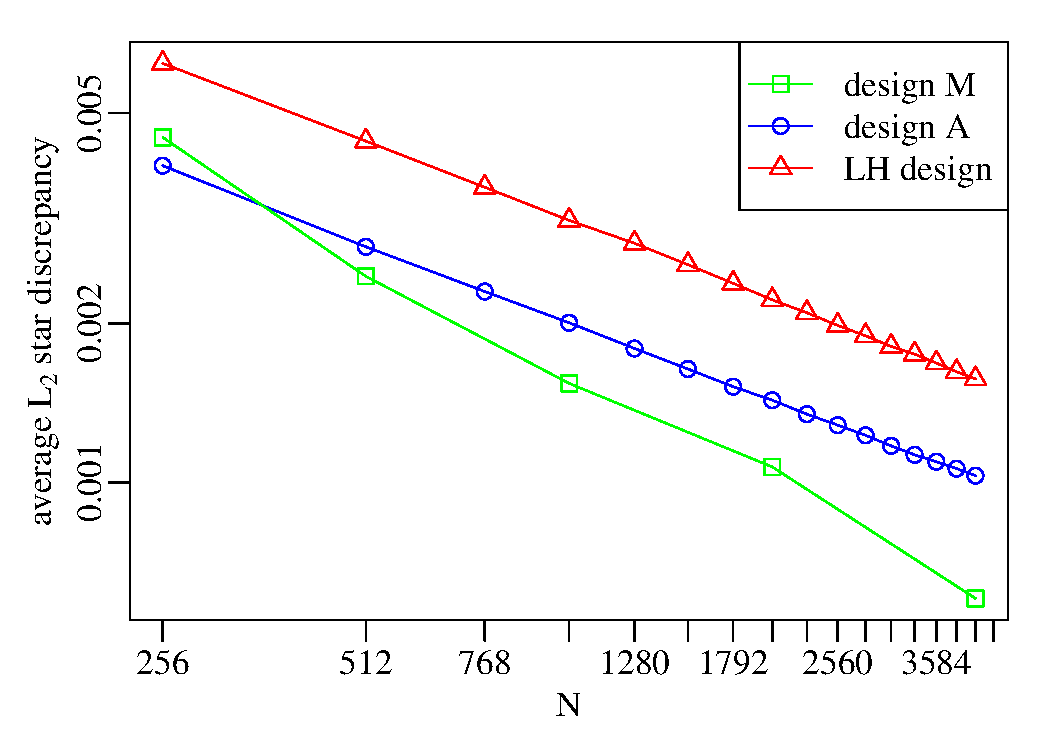
\includegraphics[scale=0.38]{discrep.pdf}
\hspace*{0.1cm}
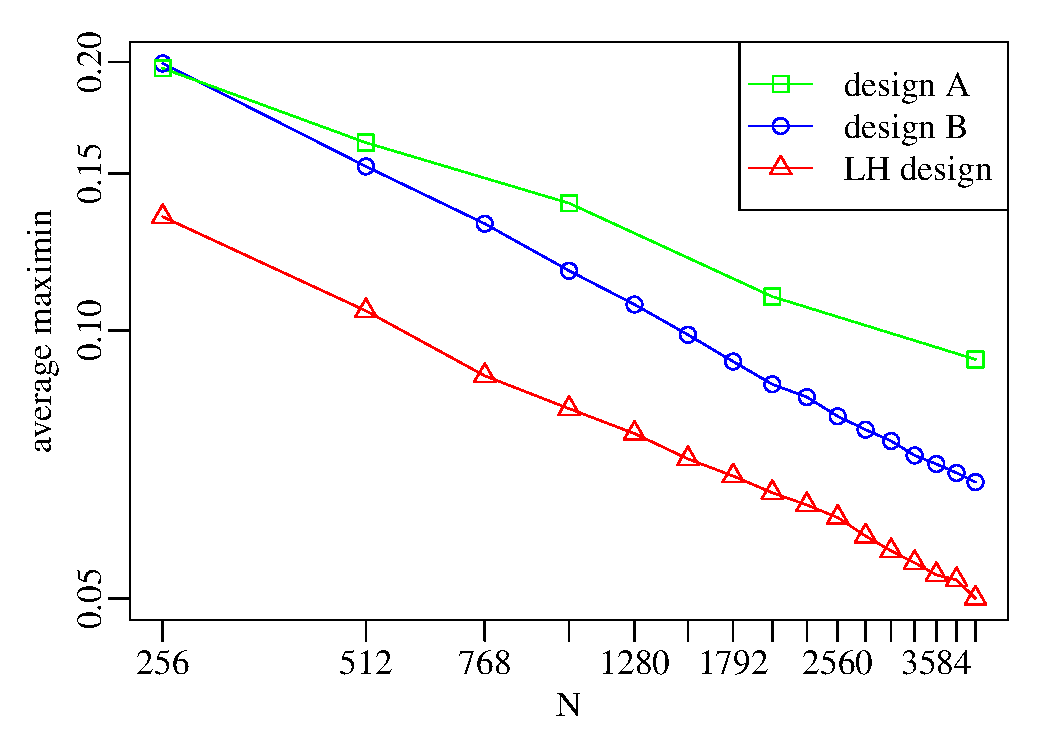
\includegraphics[scale=0.38]{mindist.pdf}
\end{figure}



%In addition to it, one can still randomize the initial Sobol' sequence using Owen's scrambling \cite{owen.scrambl}. The only requirement to keep the replication property is to apply the same scrambling to dimensions that differ by $s$ positions, i.e., same scrambling to $C_j$ and $C_{j+s}$ for all $j=1,\dots,s$.

%\label{}
% etc, etc

% The Appendices part is started with the command \appendix;
% appendix sections are then done as normal sections
% \appendix

% \section{}
% \label{}

% The Acknowledgements are an un-numbered section
\section*{Acknowledgements}
This work is supported by the CITiES project funded by the Agence Nationale de la Recherche (grant ANR-12-MONU-0020). 


\begin{thebibliography}{00}
% please try to use the bibitem system -
% the references should be in alphabetical order of authors' names.
% Articles with a single author first, author will 1 co-author next,
% then author with several co-authors;

% \bibitem{label}
% Text of bibliographic item
\bibitem{Kuo} S. Joe, F. Y. Kuo, Constructing Sobol Sequences with Better Two-Dimensional Projections, \emph{SIAM J. Sci. Comput.} 30(8), 2008, pp. 2635--2654.

\bibitem{Mara} T. A. Mara, O. R. Joseph, Comparison of some efficient methods to evaluate the main effect of computer model factors, \emph{Journal of Statistical Computation and Simulation} 78(2), 2008, pp. 167--178.

\bibitem{Matousek} J. Matou$\check{s}$ek, On the $L2$-discrepancy for anchored boxes, \emph{Journal of Complexity} 14, 1998, pp. 527-556.

\bibitem{Mckay} M. D. McKay, W. J. Conover, R. J. Beckman, A comparison of three methods for selecting values of input variables in the analysis of output from a computer code, \emph{Technometrics} 21, 1979, pp. 239--245.

\bibitem{Morokoff} W. J. Morokoff, R. E. Caflisch, Quasi-random sequences and their discrepancies, \emph{SIAM Journal on Scientific Computing} 15, 1994, pp.1251?-1279.

\bibitem{Niederreiter} H. Niederreiter, Random Number Generation and Quasi-Monte Carlo Methods, \emph{CBMS-NSF Regional Conference Series in Applied Math.} 63, SIAM,Philadelphia, PA, 1992.

\bibitem{NiederreiterXing} H. Niederreiter, C. Xing, Low-Discrepancy Sequences and Global Function Fields with Many Rational Places, \emph{Finite Fields and Their Applications} 2(3), 1996, pp. 241--273.

\bibitem{OwenScrambling} A. B. Owen, Scrambling Sobol' and Niederreiter-xing points, \emph{J. Complexity}, 14(4), 1998, pp. 466--489.

\bibitem{Saltelli} A. Saltelli, Making best use of model evaluations to compute sensitivity indices, \emph{Computer Physics Communications} 145(2), 2002, pp. 280--297.

\bibitem{Sobol1} I. M. Sobol', On the distribution of points in a cube and the approximate evaluation of integrals, \emph{USSR Computational Mathematics and Mathematical Physics} 7(4), 1967, pp. 86--112.

\bibitem{Sobol2} I. M. Sobol', Sensitivity indices for nonlinear mathematical models, \emph{Mathematical Modeling and Computational Experiment} 1, 1993, pp. 407--414.

%\bibitem{Tezuka} S. Tezuka, H. Faure, I-binomial scrambling of digital nets and sequences, \emph{J. Complexity} 19(6),2003, pp. 744--757.

\bibitem{Tissot} J. Y. Tissot, C. Prieur, A randomized orthogonal array-based procedure for the estimation of first- and second-order Sobol' indices, \emph{J. Statist. Comput. Simulation} 85, 2014, pp. 1358--1381.


\end{thebibliography}

\end{document}
